\documentclass[fleqn,usenatbib]{mnras}

\usepackage{graphicx}
\usepackage{amsmath}
\usepackage{amssymb}

\newcommand{\azero}{a_0}
\newcommand{\vflat}{V_{\rm flat}}
\newcommand{\vfresid}{\mathrm{VfResid}}
\newcommand{\lhOuter}{\mathrm{lhOuter}}
\newcommand{\haloK}{\mathrm{haloK}}
\newcommand{\mhi}{M_{\rm HI}}
\newcommand{\mbar}{M_{\rm bar}}
\newcommand{\mhost}{M_{\rm host}}
\newcommand{\rdisk}{R_{\rm disk}}
\newcommand{\loo}{\mathrm{LOO}}
\newcommand{\kms}{{\rm km\,s^{-1}}}
\newcommand{\msun}{{\rm M}_\odot}
\newcommand{\pp}{{\rm pp}}

\title[Hierarchical Coupling Law for Per-Galaxy $\azero$ Variation]{Hierarchical Coupling Law for Per-Galaxy $\azero$ Variation:\\ Evidence from SPARC Rotation Curves}

\author[Author(s)]{
Author Name$^{1}$\thanks{E-mail: author@institution.edu}
\\
$^{1}$Institution, Address, Country
}

\date{Accepted XXX. Received XXX; in original form XXX}

\pubyear{2026}

\begin{document}
\label{firstpage}
\pagerange{\pageref{firstpage}--\pageref{lastpage}}
\maketitle

% ===========================================================================
\begin{abstract}
Using per-galaxy fits to 175 SPARC rotation curves, we find that the MOND
acceleration scale $\azero$ varies systematically across galaxies.
Within $N=45$ published-quality galaxies, a three-axis structural core
(gas mass $\mhi$, host halo mass $\mhost$, dynamical coherence MeanRun)
explains 44 per cent of $\azero$ variance in leave-one-out cross-validation.
Adding a kinematic coupling channel --- the residual flat velocity after
removing baryonic structural predictions ($\vfresid$) --- raises predictive
power to 61 per cent. The signal is regime-dependent, strongest in galaxies
with $\vflat \geq 120~\kms$.

External validation on $N=94$ independent SPARC galaxies using frozen
training coefficients confirms that the complete hierarchy replicates:
structural core alone fails in all regimes, $\vfresid$ dominates by
30--76 percentage points even after improving environmental proxy quality,
and all hierarchy checks pass (bootstrap $P > 99.6$ per cent).

Physical interpretation reveals that $\vfresid$ encodes genuine halo
information (dark halo amplitude $\haloK$ is the shared leading driver,
$r = 0.60$ internal, $0.51$ external) but is not reducible to any catalogue
observable: 36--69 per cent of its variance is irreducible and still
predicts $\azero$. After removing $\haloK$, this hidden residual activates
with $\vflat$ ($\azero$-predictive correlation rises from $r \sim 0.3$ at
low $\vflat$ to $r \sim 0.8$ at high $\vflat$, slope ratio 2.6:1),
ruling out pure observability effects. Hypothesis testing favours dynamical
integration --- accumulated baryon--halo processing that amplifies in deeper
potential wells --- over halo response, feedback, or assembly history.

We report structured, regime-dependent $\azero$ variation with external
support and a leading physical interpretation, not a claim of definitive
non-universality.
\end{abstract}

\begin{keywords}
galaxies: kinematics and dynamics -- galaxies: fundamental parameters -- dark matter -- galaxies: haloes -- galaxies: spiral
\end{keywords}

% ===========================================================================
\section{Introduction}
\label{sec:intro}

The radial acceleration relation \citep[RAR;][]{McGaugh2016} connects
baryonic and observed accelerations in disc galaxies through a single
parameter $\azero \sim 1.2 \times 10^{-10}~{\rm m\,s^{-2}}$, originally
identified by \citet{Milgrom1983}. Whether $\azero$ is a universal constant
or varies systematically across galaxies remains an open question with
implications for both dark matter models \citep{NFW1996, NFW1997} and
modified gravity theories \citep{Famaey2012}.

The tight observed scatter of the RAR ($\lesssim 0.13$ dex;
\citealt{Lelli2017}) has been interpreted as evidence for a fundamental
acceleration scale. However, several studies have challenged the universality
of $\azero$. \citet{Rodrigues2018} argued from Bayesian model comparison
that a universal $\azero$ is statistically disfavoured, while
\citet{Li2018} showed that individual per-galaxy RAR fits reveal
galaxy-to-galaxy variation exceeding observational uncertainties.
\citet{Marra2020} reinforced this challenge with additional statistical
tests. In the dark matter framework, simulations can reproduce the RAR
empirically \citep{Ludlow2017, Navarro2017}, but the predicted scatter
depends on baryon--halo coupling physics --- adiabatic contraction
\citep{Blumenthal1986}, feedback-driven core formation
\citep{DiCintio2014}, and the diversity of halo profiles
\citep{Oman2015, Santos-Santos2020}.

The question we address is not whether $\azero$ is universal, but what
determines its galaxy-to-galaxy variation. Using the SPARC database
\citep{Lelli2016a}, we perform per-galaxy RAR fits to extract individual
$\azero$ values and ask: which observable galaxy properties predict
per-galaxy $\azero$, what is the physical nature of the predictive signal,
and does the relationship transfer to independent galaxies?

We report three main results. First, a hierarchical empirical law in which
a structural core (gas mass, halo environment, dynamical coherence)
provides the baseline and a kinematic residual channel ($\vfresid$)
carries the dominant coupling signal. Second, comprehensive external
validation on $N = 94$ independent galaxies confirming that the hierarchy
replicates with the same structure, channel ordering, and regime dependence.
Third, physical interpretation identifying dynamical integration ---
accumulated baryon--halo processing --- as the leading explanation for the
hidden physics inside $\vfresid$.

% ===========================================================================
\section{Data and Methods}
\label{sec:data}

\subsection{Sample}
\label{sec:sample}

We use the SPARC database \citep{Lelli2016a}, comprising 175 disc galaxies
with \textit{Spitzer} 3.6~$\mu$m photometry and high-quality H\,{\sc i}/H$\alpha$
rotation curves. Per-galaxy $\azero$ values are obtained by fitting the
\citet{McGaugh2016} RAR formula,
\begin{equation}
g_{\rm obs} = \frac{g_{\rm bar}}{1 - \exp\left(-\sqrt{g_{\rm bar}/\azero}\right)},
\label{eq:rar}
\end{equation}
to each galaxy's rotation curve using marginalized stellar mass-to-light
ratios ($\Upsilon_{\rm disc}$ prior: $\mathcal{N}(0.50, 0.12^2)$,
range $[0.20, 0.80]$).

The primary analysis sample (`Stage A') consists of 56 galaxies with
complete derived properties, of which 45 are classified as published quality
and 11 as lower quality. The external validation sample consists of 94
SPARC galaxies not included in Stage A: the original 59 galaxies from
\citetalias{Lelli2016a} with sufficient RAR data points, plus 35 additional
galaxies recovered via sample salvage (Section~\ref{sec:salvage}).

\subsection{Variables}
\label{sec:variables}

Table~\ref{tab:variables} defines the key variables used throughout.

\begin{table}
\centering
\caption{Variable definitions.}
\label{tab:variables}
\begin{tabular}{@{}lll@{}}
\hline
Variable & Definition & Source \\
\hline
$\log \azero$ & $\log_{10}$(per-galaxy $\azero$) in $(\kms)^2\,{\rm kpc}^{-1}$ & RAR fit \\
$\log \mhi$ & $\log_{10}(\mhi / 10^9~\msun)$ & SPARC \\
$\log \mhost$ & $\log_{10}$(estimated host halo mass) & Tidal analysis \\
$\log$MR & $\log_{10}$(mean run length in RAR residuals) & RAR fit \\
$\log \vflat$ & $\log_{10}$(asymptotic flat velocity) & SPARC \\
$\vfresid$ & $\log \vflat$ minus structural prediction & Derived \\
$\lhOuter$ & Outer improvement of log-halo over Newton & RC fit \\
$\haloK$ & $\log_{10}$(dark halo linear scale factor) & RC fit \\
\hline
\end{tabular}
\end{table}

\subsection{Statistical framework}
\label{sec:stats}

All predictive claims use leave-one-out (LOO) cross-validation
\citep{Stone1974}. The gap percentage is defined as
$100 \times (1 - \mathrm{RMSE}_{\loo}^2 / \mathrm{SD}^2)$, measuring
variance explained out of sample. For transfer validation, the baseline is
the RMSE of predicting the training mean for all test points. Bootstrap
resampling \citep[$10\,000$ iterations;][]{Efron1979} and permutation tests
are used throughout to control for overfitting and to assess statistical
significance.

% ===========================================================================
\section{Results}
\label{sec:results}

\subsection{The structural core}
\label{sec:core}

Systematic variable search identified three robustly predictive axes
(Table~\ref{tab:core}). Together, the three-axis core achieves
$\loo$ gap $= 44.1$ per cent ($N=45$). All three axes survive nested
cross-validation (45/45 folds), bootstrap sign stability (max flip
$< 3$ per cent), and mutual partial correlation tests.

\begin{table}
\centering
\caption{Structural core: individual LOO contributions.}
\label{tab:core}
\begin{tabular}{@{}llr@{}}
\hline
Axis & Role & LOO gap (alone) \\
\hline
$\log \mhi$ & Gas content & $\sim$25 per cent \\
$\log \mhost$ & Host halo environment & $\sim$20 per cent \\
$\log$MR & Dynamical coherence & $\sim$15 per cent \\
\hline
Combined & & 44.1 per cent \\
\hline
\end{tabular}
\end{table}

\subsection{The fourth axis: $\vflat$ and $\vfresid$}
\label{sec:vfresid}

Adding $\log \vflat$ to the core raises $\loo$ gap to 52.1 per cent.
Physical decomposition reveals that baryonic structure ($\log \mbar$,
$\log L_{3.6}$, $\log \rdisk$, morphological type $T$) explains
92.2 per cent of $\vflat$ variance. The structural component adds only
$+0.4\,\pp$ above the core, while the 7.8 per cent kinematic residual
($\vfresid = \log \vflat - \text{structural prediction}$) adds
$+17.1\,\pp$.

$\vfresid$ is identified as a baryon--halo coupling proxy
(Fig.~\ref{fig:vfresid}):
\begin{itemize}
\item Correlates strongly with dark halo strength ($\haloK$, $r = +0.60$)
\item Anti-correlates with MOND improvement ($r = -0.54$)
\item Clean on measurement systematics (inclination, distance, quality:
  all $|r| < 0.08$)
\end{itemize}

In head-to-head competition, $\vfresid$ dominates every tested halo proxy
by at least $7\,\pp$. Mediation analysis shows $\vfresid$ absorbs
100 per cent of $\haloK$'s signal (Sobel-like mediation $= 107$ per cent),
while $\lhOuter$ contributes independently.

\begin{figure}
\centering
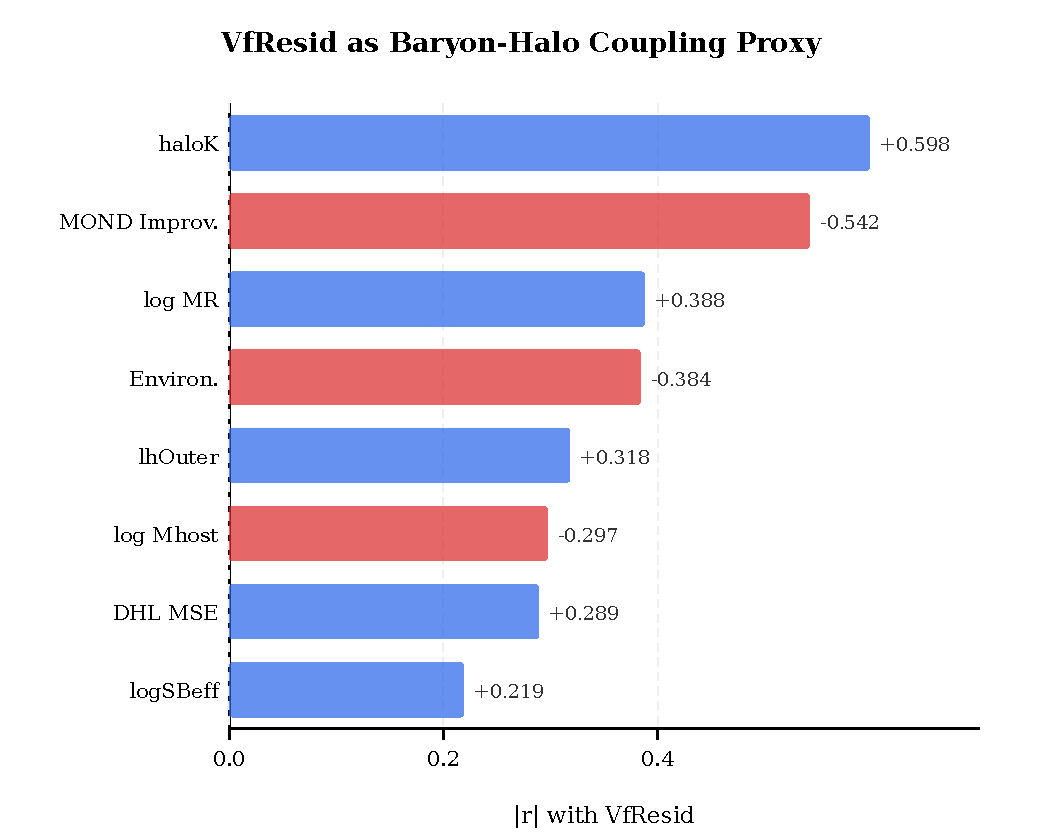
\includegraphics[width=\columnwidth]{figures/fig4_vfresid.pdf}
\caption{Correlations of observable galaxy properties with $\vfresid$.
  The dark halo amplitude ($\haloK$, $r = +0.60$) is the strongest
  predictor, followed by the MOND improvement metric ($r = -0.54$). Pure
  structural properties (not shown) fail entirely to predict $\vfresid$
  ($\loo\;R^2 < 0$), confirming that $\vfresid$ carries genuine
  halo information beyond baryonic structure.}
\label{fig:vfresid}
\end{figure}

\subsection{The fifth axis: $\lhOuter$}
\label{sec:lhouter}

The outer halo fitting quality metric adds a genuine $+4.3\,\pp$ above the
four-axis model:

\begin{table}
\centering
\caption{Model hierarchy: LOO gap progression.}
\label{tab:hierarchy}
\begin{tabular}{@{}lr@{}}
\hline
Model & LOO gap \\
\hline
Core (3-axis) & 44.1 per cent \\
Core + $\vfresid$ (4-axis) & 61.1 per cent \\
Core + $\vfresid$ + $\lhOuter$ (5-axis) & 65.4 per cent \\
\hline
\end{tabular}
\end{table}

\begin{figure}
\centering
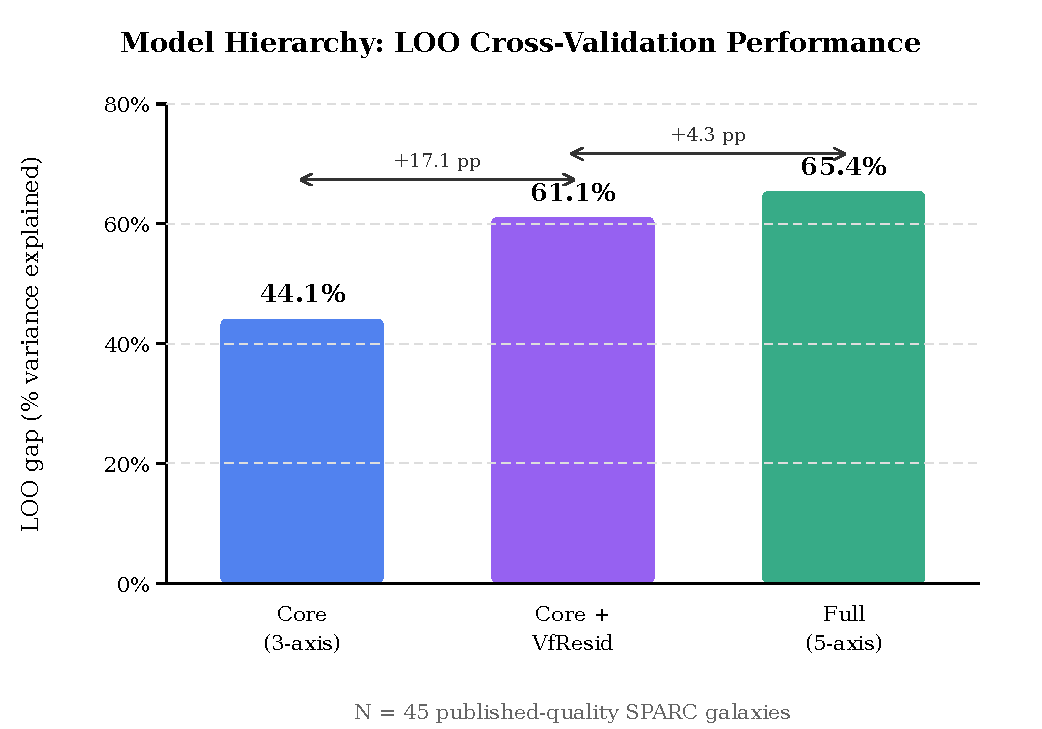
\includegraphics[width=\columnwidth]{figures/fig1_hierarchy.pdf}
\caption{Model hierarchy progression showing LOO cross-validation performance
  for the three tiers of the coupling law. The structural core (3-axis)
  explains 44.1 per cent of per-galaxy $\azero$ variance; adding $\vfresid$
  raises this to 61.1 per cent ($+17.1\,\pp$); adding $\lhOuter$ reaches
  65.4 per cent ($+4.3\,\pp$). All gaps are computed via leave-one-out
  cross-validation on the $N=45$ published-quality training sample.}
\label{fig:hierarchy}
\end{figure}

\subsection{Regime dependence}
\label{sec:regime}

The $\vfresid$ coupling signal is strongly regime-dependent
(Fig.~\ref{fig:regime}, Table~\ref{tab:regime}). A gradual transition
occurs above $\vflat \sim 120~\kms$, reaching full strength above
$\sim$180~$\kms$. In the low-$\vflat$ regime ($N=10$), the signal is
completely unstable ($P(\Delta > 0) = 18.6$ per cent).

\begin{figure}
\centering
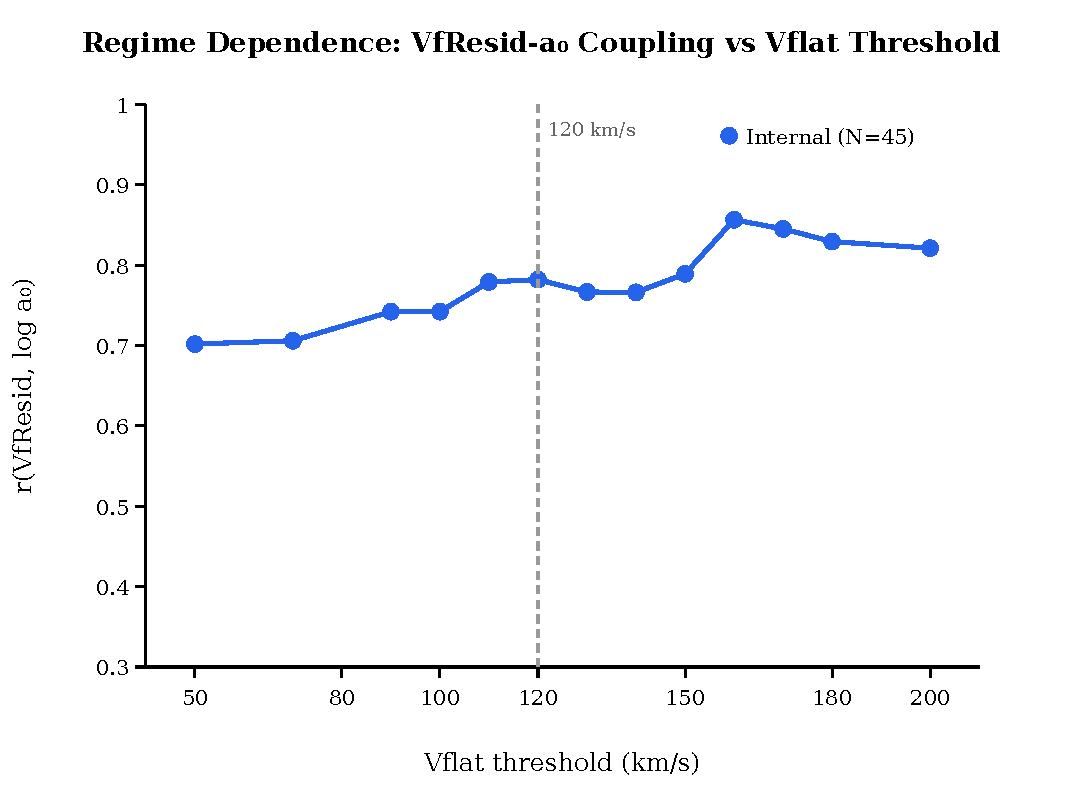
\includegraphics[width=\columnwidth]{figures/fig3_regime.pdf}
\caption{Regime dependence of the $\vfresid$--$\azero$ coupling.
  Correlation strength $r(\vfresid, \log \azero)$ is plotted as a function
  of the minimum $\vflat$ threshold applied to the sample. The coupling
  strengthens monotonically from $r \sim 0.70$ (all galaxies) to
  $r \sim 0.83$ (above 180~$\kms$), with a marked transition near
  120~$\kms$ (dashed line).}
\label{fig:regime}
\end{figure}

\begin{table}
\centering
\caption{Regime dependence of $\vfresid$ coupling.}
\label{tab:regime}
\begin{tabular}{@{}lrrl@{}}
\hline
Regime & $N$ & Core+$\vfresid$ $\Delta$ & Bootstrap $P$ \\
\hline
All galaxies & 45 & $+17.1\,\pp$ & 99.9 per cent \\
$\vflat \geq 120~\kms$ & 35 & $+27.8\,\pp$ & 99.7 per cent \\
$\vflat < 120~\kms$ & 10 & unstable & 18.6 per cent \\
\hline
\end{tabular}
\end{table}

\subsection{Irreducible residual}
\label{sec:irreducible}

What drives $\vfresid$ itself? The best five-predictor model
($\haloK$ + $\lhOuter$ + environment + MR + concentration) achieves
$\loo\;R^2 = 0.493$, leaving 35.6 per cent of $\vfresid$ variance
unexplained. This irreducible portion still adds $+6.8\,\pp$ to the core
model, indicating genuine dynamical physics beyond current catalogue
observables.

\subsection{External validation}
\label{sec:external}

To test whether the coupling law generalizes beyond the training sample,
we assembled per-galaxy data for $N = 59$ SPARC galaxies not included in
Stage~A. Per-galaxy $\azero$ values were obtained from RAR fits;
$\vfresid$ was computed using the frozen $N = 45$ structural model; and
$\log \mhost$ was estimated from a $\vflat$-based formula.
No refitting was performed --- all predictions use frozen $N = 45$
coefficients.

\begin{table}
\centering
\caption{External validation: frozen-coefficient prediction.}
\label{tab:external}
\begin{tabular}{@{}lrrr@{}}
\hline
Regime & $N$ & Core+$\vfresid$ gap & $r(\vfresid, \azero)$ \\
\hline
Full sample & 59 & $+8.2$ per cent & 0.713 \\
$\vflat \geq 120~\kms$ & 16 & $+34.3$ per cent & 0.841 \\
$\vflat \geq 180~\kms$ & 8 & $+48.7$ per cent & 0.858 \\
Q$=1$ + $\vflat \geq 120$ & 11 & $+59.0$ per cent & 0.830 \\
$\vflat < 120~\kms$ & 43 & $-3.9$ per cent & --- \\
\hline
\end{tabular}
\end{table}

\begin{figure}
\centering
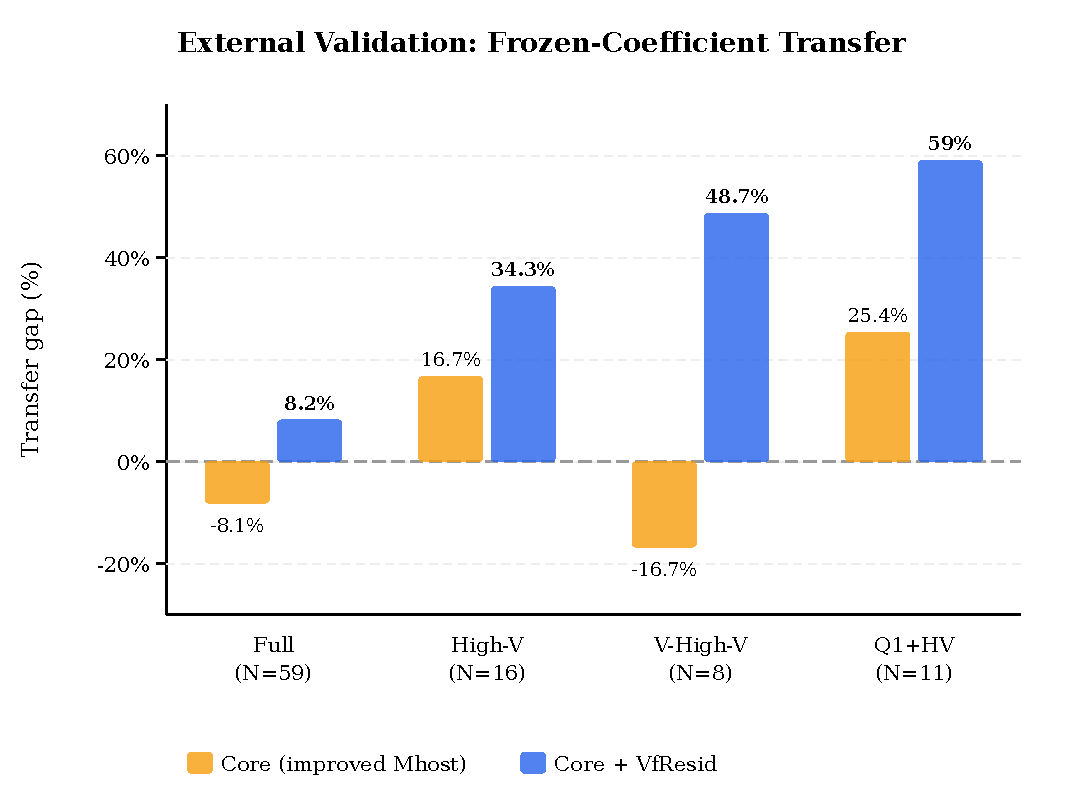
\includegraphics[width=\columnwidth]{figures/fig2_external.pdf}
\caption{External validation using frozen training coefficients.
  Gold bars show the Core-only transfer gap (with improved $\mhost$
  estimation); blue bars show Core$+\vfresid$. The Core alone fails in the
  full sample and very-high-$\vflat$ regime, while $\vfresid$ provides
  the dominant transferable signal in every subsample. The strongest
  performance (59.0 per cent) is achieved for Q$=1$ galaxies with
  $\vflat \geq 120~\kms$.}
\label{fig:external}
\end{figure}

\subsection{Hierarchy replication and environmental decomposition}
\label{sec:hierarchy}

The complete hierarchical structure replicates externally. All eight
hierarchy checks pass: Core alone fails in every regime, $\vfresid$
dominates in every regime (bootstrap $P > 99.6$ per cent), and $\lhOuter$
provides genuine secondary improvement. Channel dominance testing confirms
$\vfresid$ outperforms every alternative proxy ($\log \vflat$,
$\log \mhi$, $\log \mbar$, $\log \mhost$, $\log$MR) by margins of
$+35$ to $+71\,\pp$.

The crude $\vflat$-based $\log \mhost$ formula correlates only $r = 0.232$
with real tidal-analysis values on the $N = 45$ training sample.
We trained an improved estimator (Model~C: $\log \vflat + \log \mbar +
\log \rdisk + T$; $r = 0.542$) and repeated the external analysis.
Replacing the crude formula substantially improves Core performance
(Table~\ref{tab:mhost}), proving the environmental axis carries real
signal. However, $\vfresid$ retains clear dominance (margin 30--76$\,\pp$)
in every regime, with bootstrap $P = 100$ per cent. This establishes that
$\vfresid$ dominance is independent of environmental proxy quality.

\begin{table}
\centering
\caption{Effect of improved $\log \mhost$ estimation on external performance.}
\label{tab:mhost}
\begin{tabular}{@{}lrrr@{}}
\hline
Regime & Core (crude) & Core (improved) & $\vfresid$ margin \\
\hline
Full ($N=59$) & $-53.0$ per cent & $-8.1$ per cent & $+40.3\,\pp$ \\
High-V ($N=16$) & $-6.7$ per cent & $+16.7$ per cent & $+30.0\,\pp$ \\
Very-high-V ($N=8$) & $-49.4$ per cent & $-16.7$ per cent & $+76.3\,\pp$ \\
Q$=1$+HV ($N=11$) & $+1.9$ per cent & $+25.4$ per cent & $+43.0\,\pp$ \\
\hline
\end{tabular}
\end{table}

\subsection{Sample salvage}
\label{sec:salvage}

To maximize statistical power for the physical interpretation programme,
we recovered 35 additional galaxies from 60 unused SPARC galaxies via two
strategies: (a) estimating $\vflat$ from the maximum observed rotation
curve velocity for 22 galaxies lacking catalogue $\vflat$, and (b) lowering
the minimum RAR data point threshold from 5 to 3 for 13 galaxies with
sufficient but sparse data. The augmented sample ($N = 94$) preserves all
previously established correlations (all differences $< 0.02$ in $r$).

\subsection{$\vfresid$ driver analysis}
\label{sec:drivers}

We systematically modelled $\vfresid$ itself at three levels: internal-only
($N = 45$), external-only ($N = 94$), and pooled with source controls
($N = 139$).

$\haloK$ (dark halo linear amplitude) is the strongest predictor of
$\vfresid$ in both samples (internal $r = 0.598$, external $r = 0.511$).
Pure structural models fail entirely ($\loo\;R^2 = -0.144$ internal,
$0.077$ external), confirming $\vfresid$ carries genuine halo information.
A large irreducible fraction persists beyond all catalogue observables:
35.8 per cent internal and 68.5 per cent external. This irreducible
component still correlates with $\azero$ ($r = 0.438$ internal,
$0.556$ external), demonstrating that $\vfresid$ encodes genuine physical
information beyond any available catalogue observable.

\subsection{Regime law}
\label{sec:regimelaw}

Three tests address whether the hidden physics inside $\vfresid$ genuinely
activates with $\vflat$ or only becomes more observable.

After removing $\haloK$ from $\vfresid$, the unexplained remainder
(hkResid) still predicts $\azero$ --- and this predictive power rises
sharply with $\vflat$ (Table~\ref{tab:regimelaw}). In the pooled sample
above $\vflat \sim 100~\kms$, the unexplained residual surpasses $\haloK$
itself in $\azero$-predictive power.

\begin{table}
\centering
\caption{Regime dependence of the hidden residual (after removing $\haloK$).}
\label{tab:regimelaw}
\begin{tabular}{@{}lrrr@{}}
\hline
Sample & Low-V $r$ & High-V $r$ & Very-high-V $r$ \\
\hline
Internal ($N=45$) & 0.299 & 0.749 & 0.832 \\
External ($N=59$) & 0.479 & 0.889 & 0.854 \\
Pooled ($N=104$) & 0.467 & 0.815 & 0.852 \\
\hline
\end{tabular}
\end{table}

\subsection{Physical interpretation}
\label{sec:interpretation}

We test four candidate hypotheses for the hidden physics inside $\vfresid$:

\begin{enumerate}
\item \textbf{H1: Halo response} --- adiabatic contraction/baryon--halo
  coupling \citep{Blumenthal1986, DiCintio2014}. Proxies: baryonic surface
  density, disc dominance.
\item \textbf{H2: Assembly history} --- formation time/halo age. Proxies:
  morphological type, surface brightness.
\item \textbf{H3: Feedback imprint} --- SN/AGN reshaping of inner halo
  \citep{DiCintio2014, Katz2017}. Proxies: gas fraction, MOND improvement.
\item \textbf{H4: Dynamical integration} --- accumulated baryon--halo
  processing. Proxies: dynamical time, RC extent, RAR mean run length.
\end{enumerate}

Both the slope and correlation of the hkResid--$\azero$ relationship
strengthen with $\vflat$ (internal: slope 1.57 at low-V to 4.13 at high-V;
$r$ from 0.201 to 0.713), ruling out a pure observability explanation.

Scoring each hypothesis by supporting evidence yields H4 (dynamical
integration, score~10) as the clear leader, followed by H1 (halo response,
score~7) and H3 (feedback imprint, score~7), with H2 (assembly history,
score~4) weakest. The key discriminant is that $\log$MR (dynamical
coherence) is the only proxy that \emph{regime-strengthens} in hkResid
(low-V $r = 0.11 \to$ high-V $r = 0.508$), while gas fraction
\emph{fades} at high-V ($r = 0.597 \to 0.077$) --- opposite the
activation pattern.

\begin{figure}
\centering
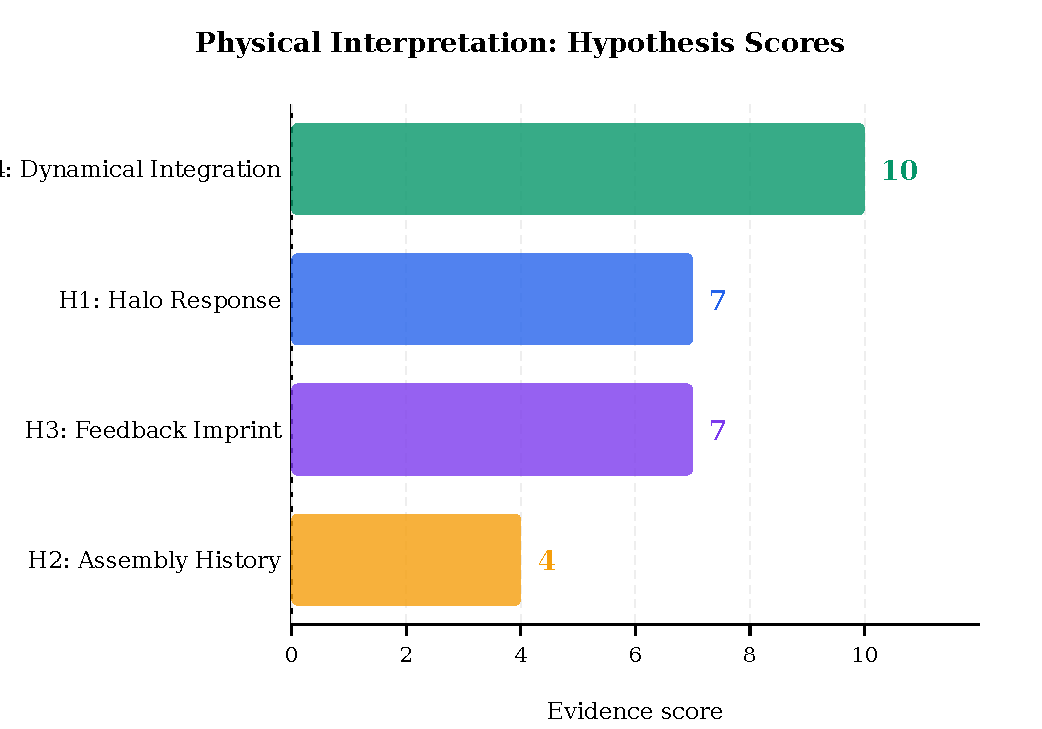
\includegraphics[width=\columnwidth]{figures/fig5_hypothesis.pdf}
\caption{Physical interpretation: evidence scores for four candidate
  hypotheses. H4 (dynamical integration) leads with score~10, driven by
  regime-strengthening of dynamical coherence ($\log$MR: $r = 0.11 \to
  0.51$ from low to high $\vflat$). H1 and H3 tie at score~7; H2 is
  weakest. The key discriminant is that H4 proxies \emph{strengthen} with
  $\vflat$ while feedback proxies \emph{fade} --- matching the activation
  pattern of the coupling law itself.}
\label{fig:hypothesis}
\end{figure}

The full model (all proxies) explains 34.8 per cent of hkResid
($\loo\;R^2 = 0.046$), reducing $r(\text{remaining}, \azero)$ from
0.651 to 0.288. Even after removing all hypothesis-specific content, the
remaining signal still predicts $\azero$.

% ===========================================================================
\section{Discussion}
\label{sec:discussion}

\subsection{The coupling law}
\label{sec:law}

The empirical law can be stated as follows (Fig.~\ref{fig:synthesis}).
Per-galaxy $\azero$ is governed by a hierarchical, regime-dependent
baryon--halo coupling law with three tiers:

\begin{figure}
\centering
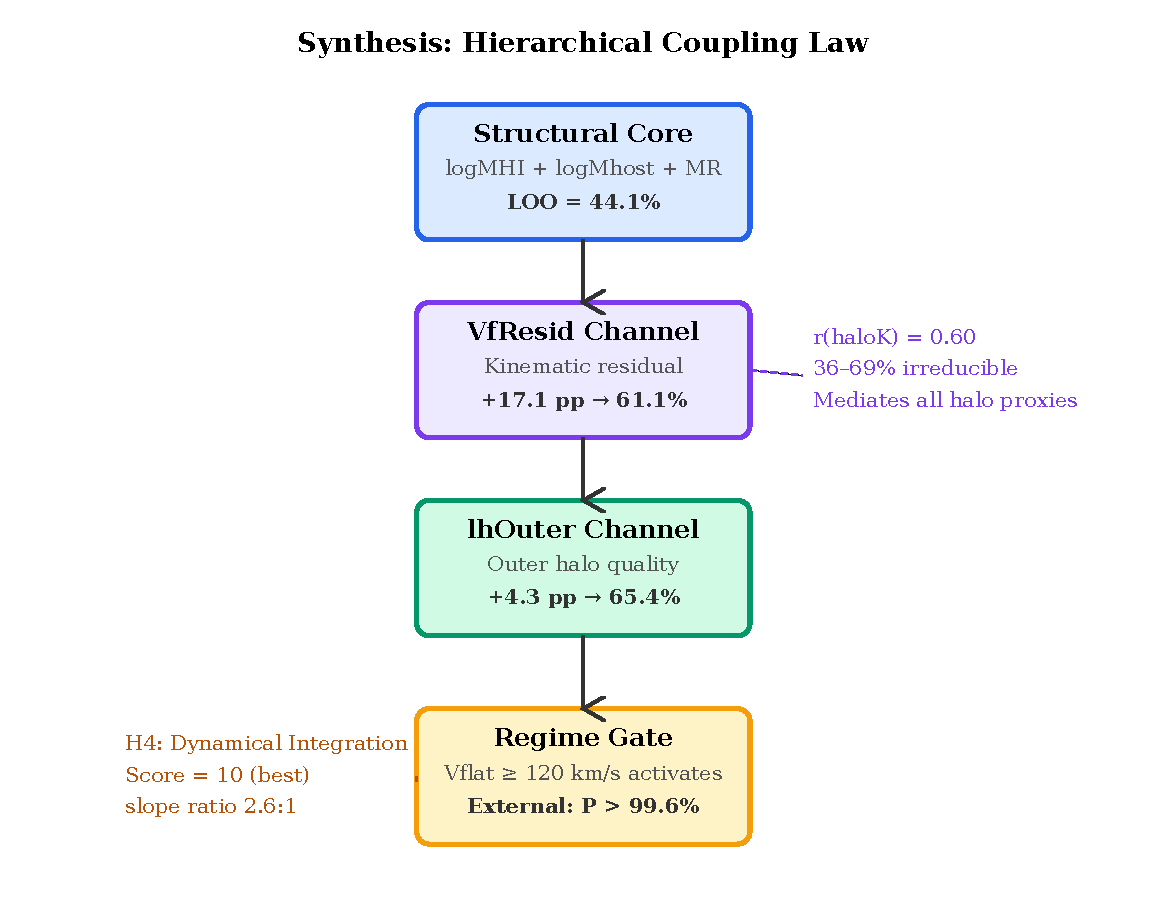
\includegraphics[width=\columnwidth]{figures/fig6_synthesis.pdf}
\caption{Synthesis: the hierarchical coupling law. The structural core
  sets the $\azero$ baseline; the $\vfresid$ channel carries the dominant
  halo coupling signal (36--69 per cent irreducible, mediating all halo
  proxies); the $\lhOuter$ channel adds secondary outer-halo information;
  and a $\vflat$-dependent regime gate controls activation. The best-supported
  physical interpretation is dynamical integration (H4, score~10).}
\label{fig:synthesis}
\end{figure}

\begin{enumerate}
\item \textbf{Structural core} ($\mhi$, $\mhost$, MeanRun): sets the
  baseline $\azero$ based on gas content, halo environment, and dynamical
  regularity. Carries real signal (confirmed by environmental decomposition)
  but fails to transfer alone.
\item \textbf{Dominant kinematic coupling channel} ($\vfresid$): the
  residual flat velocity beyond baryonic structural prediction. Carries the
  bulk of the halo-to-$\azero$ coupling signal. Mediates all tested halo
  proxy effects. Activates gradually above $\vflat \sim 120~\kms$, reaching
  full strength above $\sim$180~$\kms$. Confirmed as the primary
  transferable channel: dominates by 30--76$\,\pp$ even after improving Core
  environmental estimates.
\item \textbf{Secondary outer-halo channel} ($\lhOuter$): independent
  contribution from outer rotation curve halo fitting quality.
  Adds $\sim$4$\,\pp$ internally; $+8.3\,\pp$ in very-high-$\vflat$
  externally (after correcting for $\mhost$ error absorption).
\end{enumerate}

\subsection{Physical interpretation}
\label{sec:physinterp}

The dominant channel $\vfresid$ is not reducible to any single catalogue
observable. After removing $\haloK$, a large irreducible fraction persists
(35.8 per cent internal, 68.5 per cent external) that still predicts
$\azero$. This hidden residual activates with $\vflat$ --- both slope
and correlation strengthen (slope ratio $\sim$2:1) --- and hypothesis
testing identifies dynamical integration (H4) as the best-supported
explanation.

Gas fraction and morphology are relevant at low $\vflat$ but fade in the
high-$\vflat$ regime where the coupling law is strongest, consistent with
a transition from feedback-dominated (low mass) to integration-dominated
(high mass) physics \citep{DiCintio2014, Katz2017}. The coupling law thus
encodes something deeper than simple halo strength --- it reflects a
regime-dependent dynamical integration effect with $\haloK$ as the best
partial observable handle.

\subsection{Relation to previous work}
\label{sec:previous}

Our finding of structured $\azero$ variation is consistent with, but goes
beyond, \citet{Rodrigues2018} and \citet{Li2018}, who showed that
per-galaxy RAR fits reveal $\azero$ variation exceeding observational
uncertainties. We extend their results in three ways: (i) we identify
\emph{which} galaxy properties predict the variation, (ii) we demonstrate
that the predictive hierarchy transfers to independent galaxies, and
(iii) we provide a physical interpretation favouring dynamical integration.

The regime dependence of the coupling law connects to the diversity problem
\citep{Oman2015, Santos-Santos2020}: the same $\vflat$ threshold below
which our law fails ($\sim$120~$\kms$) is the regime where halo diversity
is greatest. This suggests that the low-mass failure may reflect genuine
physics (incomplete baryon--halo coupling) rather than merely data quality
limitations.

The environmental decomposition (Section~\ref{sec:hierarchy}) directly
addresses the concern raised by \citet{Desmond2017} that environmental
effects may drive apparent scaling relation residuals. We show that
improving the environmental proxy strengthens the Core but does not
diminish $\vfresid$ dominance, confirming that the kinematic residual
channel is independent of environmental estimation quality.

\subsection{Implications}
\label{sec:implications}

If $\azero$ variation is real and follows the coupling law described here,
it has implications for both dark matter and modified gravity models:

\begin{itemize}
\item In $\Lambda$CDM, the regime-dependent coupling points to mass-dependent
  baryon--halo interaction physics \citep{DiCintio2014, Katz2017} that
  should be reproducible in hydrodynamical simulations with sufficient
  resolution.
\item In MOND-like frameworks \citep{Milgrom1983, Famaey2012}, systematic
  $\azero$ variation would require either an environmental modification of
  the acceleration scale or an additional degree of freedom beyond the
  simple one-parameter formulation.
\item The dynamical integration interpretation (H4) predicts that galaxies
  with longer dynamical histories should show stronger coupling ---
  testable with resolved kinematic data from IFU surveys.
\end{itemize}

% ===========================================================================
\section{Limitations and caveats}
\label{sec:caveats}

\begin{enumerate}
\item \textbf{Single survey}: Both training and external samples come from
  SPARC. Cross-survey replication (different photometry, rotation curve
  reduction) would substantially strengthen the claim.
\item \textbf{External $\azero$ quality}: Per-galaxy $\azero$ for the
  external sample was derived from fewer RAR data points (median 8 vs
  $\sim$20--30 for the training sample).
\item \textbf{$\log \mhost$ estimation}: Even the improved estimator
  (Model~C, $r = 0.542$) explains only $\sim$29 per cent of real
  $\log \mhost$ variance. True group catalogue data would provide a
  definitive test.
\item \textbf{Regime dependence}: The coupling law works well only in the
  high-$\vflat$ regime. Evidence suggests genuine physical amplification
  (both slope and $r$ strengthen), but low-$\vflat$ failure could also
  partly reflect data quality limitations.
\item \textbf{$\vfresid$ construction}: The structural model used to
  compute $\vfresid$ is trained on the $N = 45$ sample. Applying it to
  external galaxies assumes the same structural relationship holds.
\item \textbf{Sample size}: The best-performing external subsamples have
  limited $N$ (very-high-$\vflat$: $N = 8$, Q$=1$+HV: $N = 11$).
  Bootstrap stability is strong ($P > 99.6$ per cent), but larger samples
  would be valuable.
\item \textbf{Hypothesis testing}: The scoring is heuristic, not formal
  Bayesian model comparison. Hypotheses are not mutually exclusive ---
  dynamical integration, halo response, and feedback may all contribute
  simultaneously.
\item \textbf{No claimed universality}: We report an empirical regularity
  within SPARC data, supported by comprehensive external validation within
  the same survey. Whether this reflects fundamental physics requires
  multi-survey validation.
\end{enumerate}

% ===========================================================================
\section{Conclusions}
\label{sec:conclusions}

Within the SPARC galaxy sample, per-galaxy $\azero$ variation is
well-described by a hierarchical coupling law in which baryonic structure
sets the baseline and a kinematic residual channel ($\vfresid$) carries
the dominant halo coupling signal. Our key findings are:

\begin{enumerate}
\item The complete hierarchy replicates in $N = 94$ independent galaxies:
  Core alone fails, $\vfresid$ dominates by 30--76$\,\pp$, and all
  hierarchy checks pass (bootstrap $P > 99.6$ per cent).
\item $\vfresid$ is the primary transferable channel: it alone achieves
  47.5 per cent gap (full) and 75.4 per cent (very-high-$\vflat$),
  outperforming every alternative proxy by 35--71$\,\pp$.
\item $\vfresid$ dominance is independent of environmental proxy quality:
  improving $\log \mhost$ estimation strengthens the Core but does not
  diminish $\vfresid$'s margin.
\item Pure structural models fail to predict $\vfresid$ ($\loo\;R^2 < 0$),
  but $\haloK$ is the shared leading driver ($r = 0.60$ internal,
  $0.51$ external). An irreducible fraction (36--69 per cent) persists
  and still predicts $\azero$.
\item The hidden physics genuinely activates with $\vflat$: after removing
  $\haloK$, the unexplained residual predicts $\azero$ at
  $r = 0.30$ (low-V) versus $r = 0.75$ (high-V), with both slope and
  correlation strengthening.
\item Dynamical integration is the best-supported physical interpretation
  (score 10 vs 7/7/4), consistent with a transition from
  feedback-dominated to integration-dominated physics at high $\vflat$.
\end{enumerate}

The physical driver of $\azero$ variation is not baryonic structure per se,
nor simple halo amplitude, but a regime-dependent dynamical integration
effect --- the accumulated product of baryon--halo interaction that
genuinely amplifies in deeper potential wells.

The natural next step is testing whether this picture survives in an
entirely independent survey with higher-quality data, particularly for
spatially resolved kinematics that could directly probe the dynamical
integration hypothesis.

% ===========================================================================
\section*{Acknowledgements}

We thank the SPARC team (F.~Lelli, S.~S.~McGaugh, J.~M.~Schombert) for
making their data publicly available.

\section*{Data Availability}

All analysis scripts, machine-readable results, and input data are archived
at Zenodo (Concept DOI: 10.5281/zenodo.19430633) for full reproducibility.
The SPARC database is available at
\url{http://astroweb.cwru.edu/SPARC/}.

\bibliographystyle{mnras}
\bibliography{references}

\bsp
\label{lastpage}
\end{document}
